%% Anhang nit Impulsmatrixelementen und eff. Massen als Funktion der BGR
%% Time-stamp: <1999-03-04 14:14:22 ralf>

\chapter{Ergebnisse in Abh"angigkeit von $\Delta E_{\mathrm{BGR}}$}
\label{cha:ergeb-BGR}

In Kap.~\ref{sec:ergeb} haben wir die Ver"anderung der Impulsmatrixelemente
zwischen Leitungsband- und Valenzband-Zust"anden sowie die effektiven Massen
der untersten beiden Leitungsb"ander als Funktion des Potentialmatrixelements
\V{11} dargestellt. Diese Darstellung ist sinnvoll, da \V{11} des einzige
freie Parameter in dem von uns gew"ahlten Modell ist. Allerdings ist dieses
Potentialmatrixelement kaum me"sbar. Deshalb stellen wir auf den folgenden
Seiten diese Ergebnisse nochmals dar, diesmal aber als Funktion der
Bandl"uckenabsenkung $\Delta E_{\mathrm{BGR}}$. Die Diskussion in
Kap.~\ref{sec:ergeb} kann sinngem"a"s "ubertragen werden.

\begin{figure}[htb]
  \centering 
  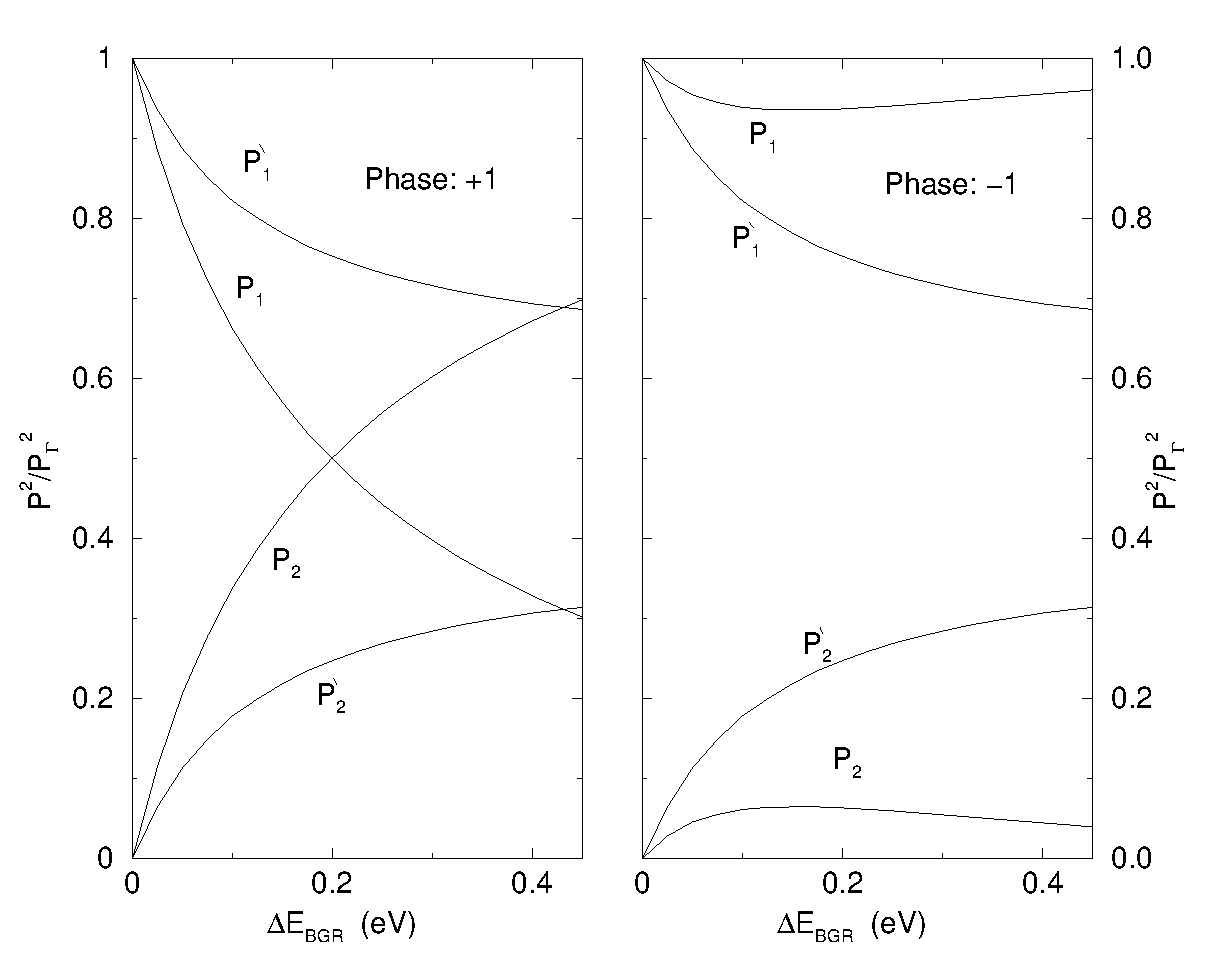
\includegraphics[width=\textwidth]{P.oV11.eps}
  \caption{Betragsquadrat der Impulsmatrixelemente aus
  Gl.~\eqref{eq:neu-k.p-H} f"ur positives und negatives relatives Vorzeichen
  von \V{11} und \V{35} in Einheiten von $|\PG|^{2}$.} 
  \label{fig:P-me.oV11}
\end{figure}


\begin{figure}[htb]
  \centering
  \includegraphics[width=\textwidth]{masses.G.oV11.eps}
  \caption{Effektive Massen von \bGCB (\GCB) f"ur positives und negatives
    relatives Vorzeichen von \V{11} und \V{35}.} 
  \label{fig:m*-GCB.oV11}
\end{figure}


\begin{figure}[htb]
  \centering
  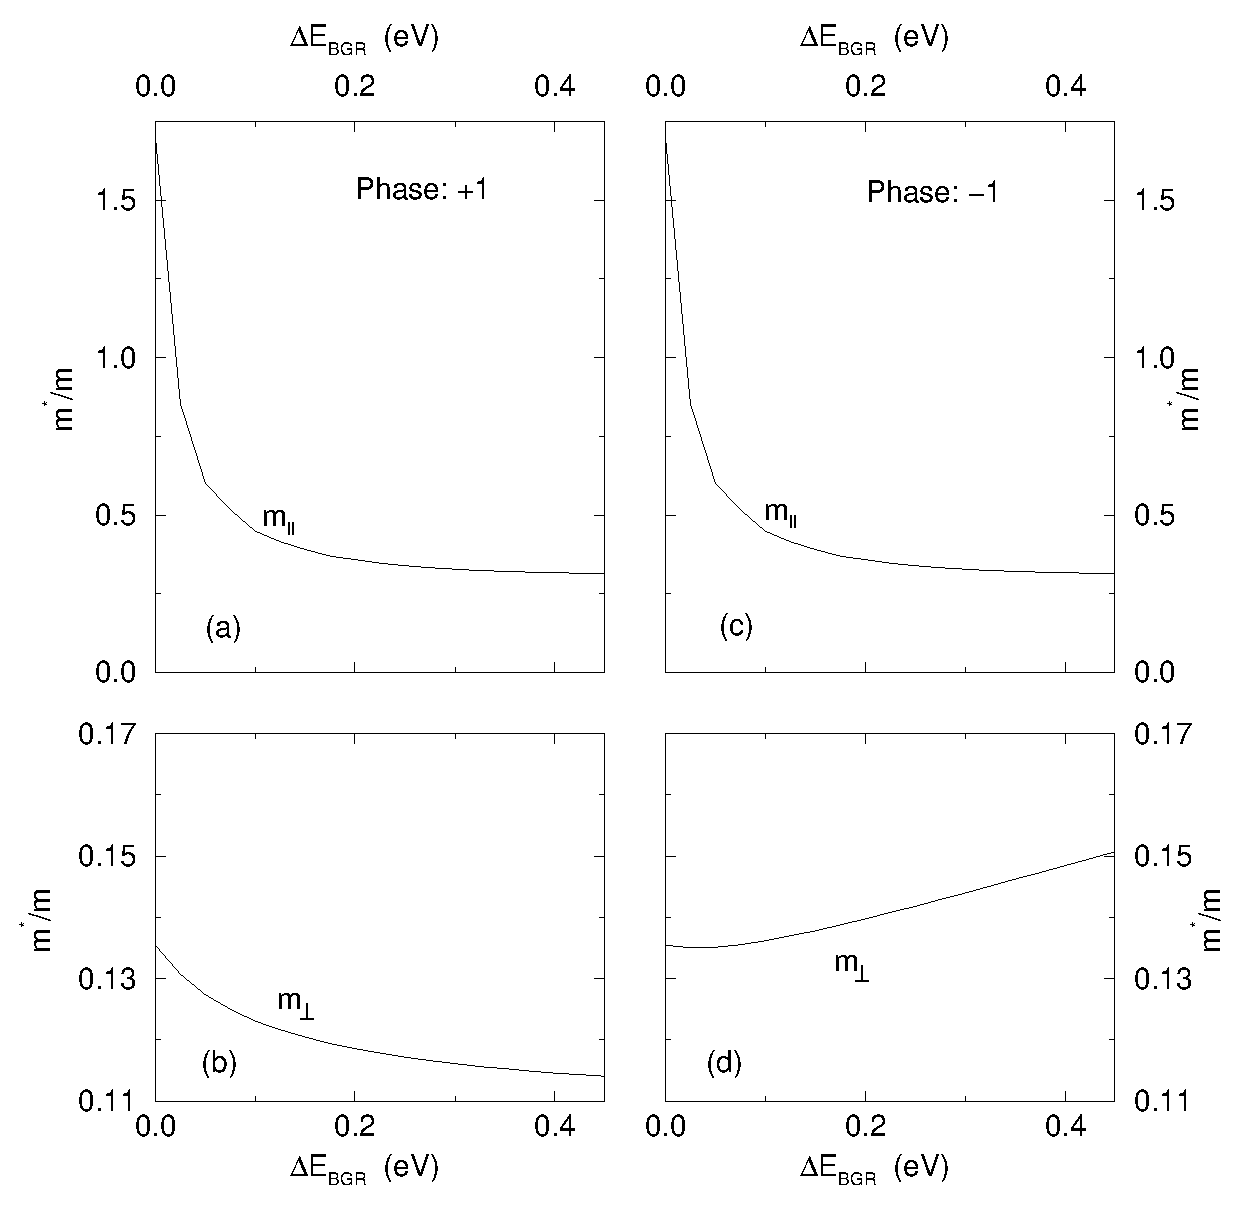
\includegraphics[width=\textwidth]{masses.L2.oV11.eps}
  \caption{Effektive Massen von \bGCB (\LCB) f"ur positives und negatives
    relatives Vorzeichen von \V{11} und \V{35}.} 
  \label{fig:m*-LCB.oV11}
\end{figure}



%%% Local Variables: 
%%% mode: latex
%%% TeX-master: "diplom"
%%% End: 
